% Graph

\begin{itemize}
    \item \textbf{Node/ Vertex:} Object with name and data (in context of molecules: the atoms)
    \item \textbf{Edge:} Connection between two vertices (in context of molecules: the bond)
    \begin{itemize}
        \item Can be weighted (in context of molecules: single bond and double bond)
        \item Can be directed 
    \end{itemize}
    \item \textbf{Graph:} Collection of nodes and edges
    \begin{center}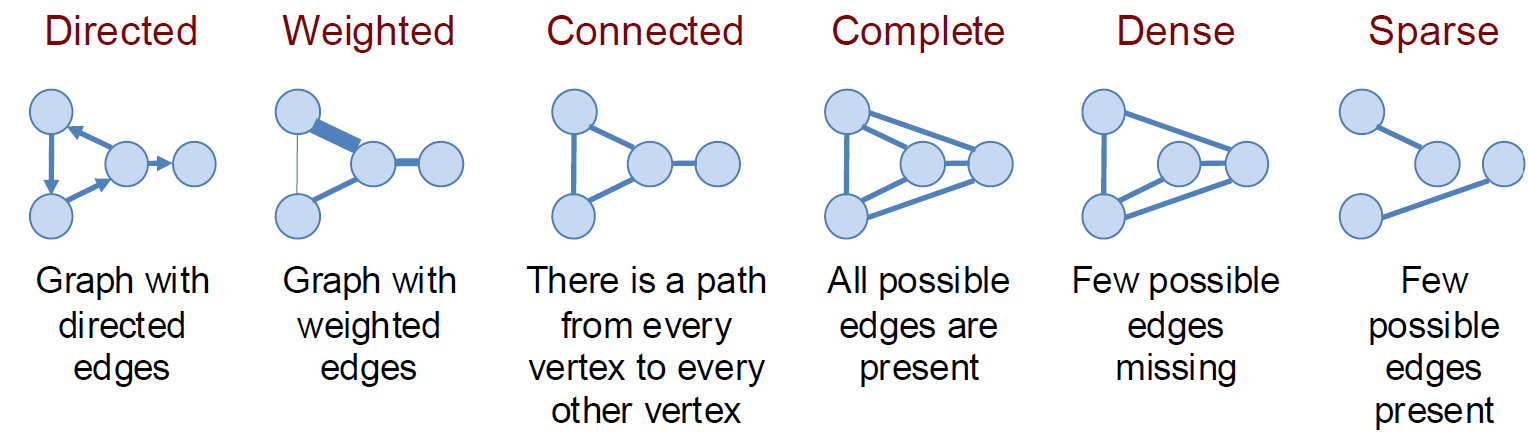
\includegraphics[width=0.85\textwidth]{img/graphs/DifferentGraphs.png}\end{center}
    \item \textbf{Valence of degree of vertex:} Number of edges a vertex lies on (in context of molecules: valence)
    \item \textbf{Adjacent vertices:} Vertices connected by an edge (in context of molecules: neibouring atoms)
    \item \textbf{Path:} List of distinct vertices in which successive vertices are connected by edges
    \begin{itemize}
        \item Simple Path: path with no vertex occurring twice
        \item Cycle Path: simple path of which first and last vertex are the same
    \end{itemize}
    \begin{center}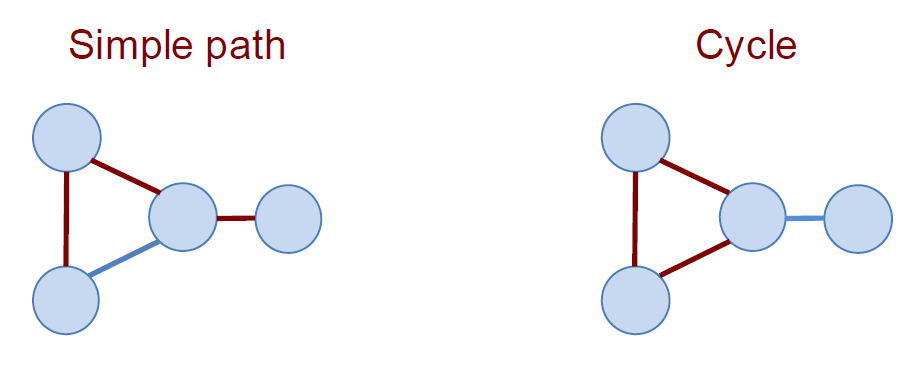
\includegraphics[width=0.85\textwidth]{img/graphs/PathGraphs.png}\end{center}
    \item \textbf{Trees:} (in graph theory)
    \begin{itemize}
        \item \textbf{Tree:}
        \item \textbf{Ordered Tree:} tree with order in the children nodes
        \item \textbf{Binary Tree:} ordered tree in which each non-terminal node has exactly two children
        \item \textbf{Binary Search Tree:} ordered binary tree with left-to-right order
        \item \textbf{Heap:} ordered binary tree with top-to-bottom order
    \end{itemize}
\end{itemize}

\subsection{Representations of graphs}

\begin{table}[H]
    \centering
    \begin{tabular}{p{30mm} | p{50mm} | p{50mm}}
        \toprule
        \textbf{Function} & \textbf{Adjacency list} & \textbf{Adjacency matrix} \\
        \midrule
        \lstinline|size()| & Easy, size of a vector & Easy, soize of a vector \\
        \midrule
        \lstinline|isConnected()| & Difficult, search in linked list & Easy, direct access \\
        \midrule
        \lstinline|getNeighbours()| & Easy, copy of linked list & Difficult, search in row \\
        \midrule
        \lstinline|addEdge()| & Easy, append linked list & Easy, set matrix element to 1 \\
        \bottomrule
    \end{tabular}
\end{table}

\subsubsection{Adjacency list}

\lstinputlisting[language=C++]{src/graphs/graph_list.cpp}

\subsubsection{Adjacecy matrix}

\lstinputlisting[language=C++]{src/graphs/graph_matrix.cpp}

\subsection{Searching a graph}

\subsection{Minimum spanning trees}

\subsection{Single-source shortest paths}

\subsection{All-pair shortest paths}